% Created 2021-10-10 Sun 18:03
% Intended LaTeX compiler: pdflatex
\documentclass[a4paper,fontsize=11pt]{article}
\usepackage[utf8]{inputenc}
\usepackage[T1]{fontenc}
\usepackage{graphicx}
\usepackage{grffile}
\usepackage{longtable}
\usepackage{wrapfig}
\usepackage{rotating}
\usepackage[normalem]{ulem}
\usepackage{amsmath}
\usepackage{textcomp}
\usepackage{amssymb}
\usepackage{capt-of}
\usepackage{hyperref}
\usepackage[T1]{fontenc}
\usepackage[sfdefault]{biolinum}
\usepackage[activate={true,nocompatibility},final,tracking=true,kerning=true,spacing=true,factor=1100,stretch=10,shrink=10]{microtype}
\usepackage[dutch]{babel}
\usepackage{listings}
\usepackage{float}

\microtypecontext{spacing=nonfrench}

\author{Sil Vaes en Maarten Evenepoel}
\date{\today}
\title{Verslag BDA opdracht 2}
\hypersetup{
 pdfauthor={Sil Vaes en Maarten Evenepoel},
 pdftitle={Verslag BDA opdracht 2},
 pdfkeywords={},
 pdfsubject={},
 pdfcreator={Emacs 29.0.50 (Org mode 9.4.6)}, 
 pdflang={English}}
\begin{document}

\maketitle
\setlength\parindent{0pt}

Voor dit project was het de bedoeling om de topic drift binnen een gegeven wetenschappelijk onderzoeksveld doorheen de tijd te bestuderen. Wij hebben ervoor gekozen om voor deze opdracht de topic drift binnen het onderzoeksveld rond Data Mining te bestuderen.

Het programma moet gerund zoals te zien in listing \ref{lst:run}, waar de dataset file en chunk size als argumenten mee moeten gegeven worden.
Het programma zal dan de dataset file uitlezen, de tuples in een pickle file saven om bij de volgende run de dataset niet helemaal te moeten processen.
Daarna zal het programma de elbow grafieken maken en uiteindelijk de daadwerkelijke clustering met het k-means algoritme.

\begin{lstlisting}[caption={KMeans output},label={lst:run},breaklines]
python main.py <dataset_file> <chunk_size>
\end{lstlisting}

\section{Aanpak}

Om dit probleem op te lossen hebben we gebruik gemaakt van het k-means clustering algoritme. Het idee is om artikels uit de brondata samen te clusteren wanneer deze op elkaar gelijken op basis van de titels van de artikels. Een cluster stelt in dit geval een verzameling artikels voor die op elkaar lijken, en dus wellicht over eenzelfde of gelijkaardig topic gaan. Als we dit dan doen door artikels in periodes van 15 jaar te beschouwen en dan te clusteren, krijgen we een overzicht van de verschillende topics die voorkomen in elke periode van 15 jaar. Met deze informatie kunnen we vervolgens dan ook de topic drift observeren van topics binnen data mining doorheen de tijd. \\

Vooraleer we effectief data kunnen clusteren is er wat pre-processing nodig bij het inladen van de data. We gaan immers niet werken met de gehele dblp.xml dataset, maar enkel met de Data Mining gerelateerde artikels. De eerste stap die we toepassen is dan ook het extracten van enkel de data mining gerelateerde artikels uit de brondata. Dit doen we door de artikels te filteren op hun key, en te controleren of de key een van de volgende values bevat, zoals gegeven in de opgave: KDD, PKDD, ICDM, SDM. We hebben ervoor gekozen de dataset te filteren door gebruik te maken van regex. Normaal gezien is dit not-done, maar omdat er eenvoudig gekeken moet worden tussen twee tags is dit hier wel gepast.\\

Vervolgens voeren we een feature extraction uit op de titels van de overblijvende documenten met behulp van een pipeline bestaande uit een \hyperlink{https://scikit-learn.org/stable/modules/generated/sklearn.feature_extraction.text.HashingVectorizer.html}{hashing vectorizer} en een \hyperlink{https://scikit-learn.org/stable/modules/generated/sklearn.feature_extraction.text.TfidfTransformer.html}{tf-idf transformer}. De hashing vectorizer vormt de tekst om in een matrix van het voorkomen van een token. Daarna berekent tf-idf transformatie het belang van iedere token. Tf-idf is niet gewoon de rauwe termfrequentie, dit zou niet zo informatief zijn, maar houdt ook rekening met algemeen veelvoorkomende termen die in principe niet zo van belang zijn in het totaalplaatje van dit project. \\

We hebben ervoor gekozen om de hashing vectorizer te gebruiken in plaats van een count vectorizer of de gewone \hyperlink{https://scikit-learn.org/stable/modules/generated/sklearn.feature_extraction.text.TfidfVectorizer.html}{tf-idf vectorizer} omdat deze meer schaalbaar is. De hashing vectorizer heeft natuurlijk ook nadelen. Er kunnen collision optreden en de inverse transformatie valt niet te berekenen. \\

Dus de pipeline die we gebruiken returned voor elk artikel een matrix aan features behorende tot het betreffende artikel. Dit wil zeggen dat elk artikel dus wordt voorgesteld door een matrix aan numerieke vectors of die het belang van verschillende gemeten features in de titels voorstelt. Het k-means algoritme dat we hierop volgend gebruiken kan deze features gebruiken om de onderlinge afstand tussen artikels tijdens het clusteren te helpen bepalen. \\

Wanneer we gebruik maken van k-means moeten we op voorhand twee parameters beslissen, namelijk welke afstandsdefinitie we gebruiken, en in hoeveel clusters we de data willen laten opdelen door het algoritme. In onze implementatie maken we gebruiken van de standaard afstandsdefinitie die ingebakken zit in de kmeans module van sklearn, dus de euclidische afstand tussen de feature matrices die de verschillende artikel titels voorstellen. Daarnaast moeten we ook beslissen in hoeveel clusters we de data willen opdelen. Hiervoor bestaan verschillende methoden.
Wij hebben ervoor gekozen om dit manueel met het ``Elbow Criterion'' te doen. Soms waren deze grafieken redelijk onduidelijk, zeker bij het interval van 1960 tot 1975. Dit komt waarschijnlijk door het kleine aantal artikels in het interval. Ook hebben we geprobeerd het DBSCAN algoritme te gebruiken. Om resultaten te verkrijgen en om te guessen hoeveel cluster centers we zouden hebben. Na het algoritme wat te gebruiken en te spelen met de parameters kregen we hier geen goede resultaten uit. Uit de visualitie na reductie met PCA en t-SNE kregen we geen goede clusters en de top artikels om de topics te bepalen is ook moeilijk te bepalen met DBSCAN omdat er niet echt een notie is van afstand, enkel dichtheid van datapunten. Dus hebben we besloten deze straat te verlaten en gewoon verder te gaan met het ``Elbow Criterion''.

% Wij hebben ervoor gekozen het DBSCAN algoritme te gebruiken om het juiste aantal clusters voor elke decade die we gaan clusteren te bepalen. 
% TODO: DBSCAN procedure hier uitleggen

Tot slot kunnen we overgaan tot het effectief clusteren van data. Zoals eerder gezegd beschouwen we de inputdata in periodes van 15 jaar. Ook laten we de verschillende periodes die we beschouwen overlappen met een overlap van 5 jaar. Concreet gaan ge we dus data clusteren over volgende periodes: 1960-1975, 1970-1975, ..., 2010-2025. Per tijdesperiode berekenen we dan zoals eerder gezegd de nodige aantal clusters met het DBSCAN algoritme en voeren we kmeans op de data in de betreffende tijdsperiode uit. 

\section{Resultaten en Output}

We hebben ons programma uitgevoerd op de gehele DBLP dataset. Verder is het programma uitgevoerd op een machine met een Intel Core i5-4690K@4.3GHz in combinatie met 16GB DD3 Dual Channel memory. Het gebruikte besturingssysteem was Ubuntu 21.10. Overigens zagen we dat het piek geheugenverbruik stijgt tot slechts 1GB. Dit komt omdat we de DBLP dataset verwerken in chunks van 1GB, en de selectie artikels die over Data Mining gaan kleiner is dan 1GB. De gemeten runtime van het programma bedraagt 2 min en 12 sec. De output die gegeven wordt is telkens het aantal clusters per tijdsperiode, en enkele representatieve artikels binnen elke cluster binnen de bijhorende tijdsperiodes. De bekomen output is te vinden in appendix \ref{sec:output}. \\

In figuur \ref{fig:elbow} zijn ook de elbow grafieken van elk tijdsinterval te zien. Deze worden verder besproken in de discussie hieronder.

\begin{figure}[H]
  \centering
  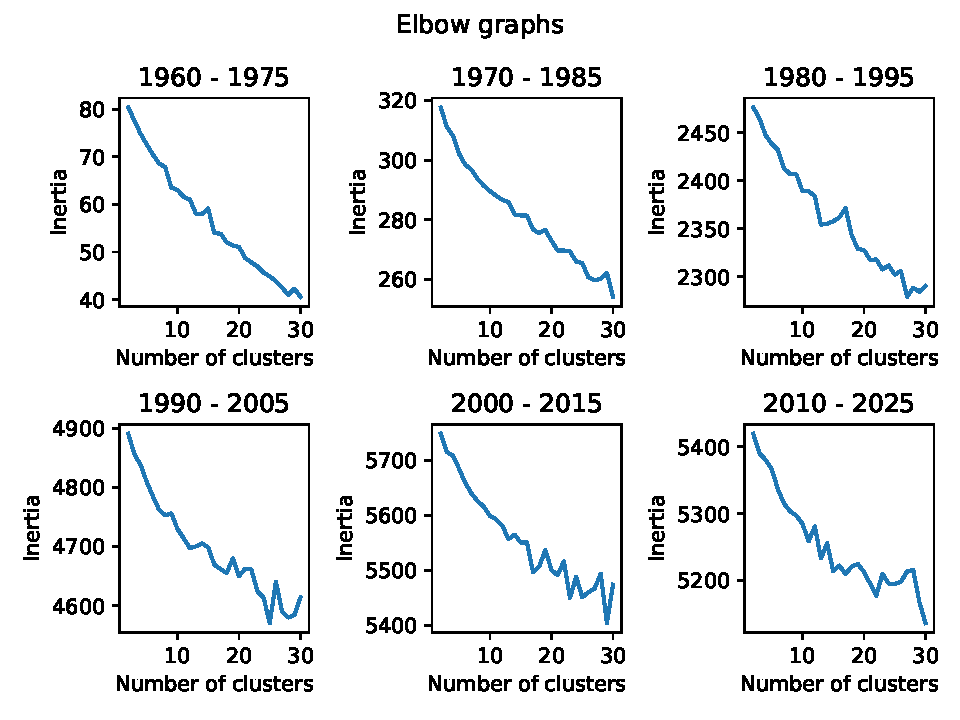
\includegraphics[width=\textwidth]{elbow.pdf}
  \caption{Elbow grafieken van alle tijdsintervallen.}
  \label{fig:elbow}
\end{figure}

\subsection{Bespreking van de resultaten}
 
We hebben k-means 6 keer uitgevoerd, telkens op periodes van 15 jaar gaande van 1960-1975 t.e.m. 2010-2025. We zien dat er in de eerste twee tijdsperiodes relatief weinig artikels aanwezig waren (88 en 328 artikels respectievelijk), wat het in de eerste plaats al onwaarschijnlijker maakt dat er zeer sterk onderscheidbare clusters zouden te vinden zijn.
Ook zaten hier veel titels zoals ``Editor's Notes'' en ``Title, Contents'' die niet interessant waren voor deze opdracht.
Deze zijn er dan ook uitgefilterd met een blacklist. Hierdoor zijn nog wat entries weggevallen uit het tijdsinterval 1960-1990 want deze waren hier voornamelijk aanwezig.
Deze zijn niet allen uitgefilterd, zo is er in het interval 1960-1975 nog steeds een cluster aanwezig die een ``Call for Papers'' representeerd en dus niet echt relevant is.
We hebben dit ook geprobeerd op te lossen door custom stopwords toe te voegen, maar dit deed niet veel en kregen we soms lege titels.
Wij waren van mening dat soms wat minder relevante entries beter zijn dan lege. \\

De 3 laatste tijdsperiodes (1990-2005 t.e.m. 2010-2025) tonen een beter representatief resultaat.
Ook het aantal vereiste clusters is hier iets groter, hier 14, 15 en 16, en dus ook evenveel verschillende topics. Om er een voorbeeld uit te halen: cluster 1 uit periode 2000-2015 lijkt vooral artikels te bevatten over data management, wat op het topic data management lijkt te wijzen voor deze cluster. \\

Omdat er van 1960 tot en met 1980 niet veel entries zijn gaan we deze hier niet bespreken. Hieronder bespreken we de belangrijkste observaties uit het clusteren:

\begin{itemize}
\item Van 1980 - 1995 zijn vooral de topics over semantic data, query optimization en processing, concurrency en object-oriented/temporal databases belangrijk.
\item Van 1990 - 2005 zijn opnieuw object-oriented/temporal databases en query optimization belangrijk. Er komen join algoritmes en web services bij. Ook zien we de opkomst van XML.
\item Van 2000 - 2015 zien we XML, join algoritmes en het web terugkomen. Wat we nog niet hebben gezien zijn de topics indexing en higher dimensional data. Wat ook interessant is, is de opkomst van het topic privacy.
\item Van 2010 - 2025 zien we veel over graphs en graph databases. Ook is er een cluster over big data en machine/deep learning, wat uiteraard vandaag de dag ook een belangrijke thema's zijn. Ook komt de topic privacy terug.
\end{itemize}

Het elbow criterion was niet ideaal zoals te zien is in figuur \ref{fig:elbow} hierboven. We hebben geprobeerd dit toch goed te krijgen door wat parameters van de pipeline en k-means te veranderen, maar het resultaat bleef echter hetzelfde of we kregen zelf nog meer noise. De parameters waarmee we het resultaat wilden aanpassen waren de shingles, of word-nGrams, van de hashing vectorizer, het aantal features van de hashing vectorizer, hoeveel keer het k-means algoritme moet runnen met een random seed en het maximum aantal iteraties van het k-means algoritme. \\

We hebben ook nog gekeken om misschien gebruik te maken van LDA, maar het resultaat van k-means bleek toch goed te zijn als we de topics bestudeerden. En we kwamen redelijk laat op het idee om LDA te gebruiken. 

% Een neveneffect dat we opnieuw waarnemen is dat er ook clusters worden gevormd op basis van features die niet topic gerelateerd zijn.
% Een voorbeeld is cluster 0 uit de periode 2000-2015.
% Deze cluster lijkt te zijn gevormd op basis van de feature dat alle titles woorden bevatten die met een liggend streepje zijn verbonden.
% Dit heeft uiteraard niets met data mining te maken. Dit is ook een fout die met wat data cleaning mogelijks voorkomen had kunnen worden.


\section{Conclusie}
Uit de resultaten valt op dat de clustering in principe wel goed werkt.
Het is duidelijk dat het programma correct artikels gaat samen clusteren op basis van tekstuele features in de titels.
Echter, het is moeilijk features uit de titels te extracten die effectief aan de semantiek van de artikels gerelateerd zijn en niet louter over tekstuele eigenschappen gaan (zoals het voorkomen van liggende streepjes, voorkomen van woordgroepen als "Editor's Notes.", etc..).
We denken hierdoor dat het gebruiken van titels van artikels niet het meest optimale onderdeel van een artikel is om te gebruiken voor het clusteren.
Het zou beter zijn moest de input data bijvoorbeeld voor elk artikel een aantal tags bevatten over waar het artikel over gaat.
Dit zou wellicht zorgen voor een veel accuratere clustering voor de opgestelde probleemstelling. Een ander alternatief zou zijn om features uit de volledige inhoud van de tekst van de artikels te halen, en niet enkel uit de titels.
Echter zijn in de DBLP dataset die we gebruikt hebben noch tags noch de effectieve inhoud van de artikels beschikbaar en konden we deze hypothese dan ook niet uittesten. 

% \begin{figure}[H]
%   \centering
%   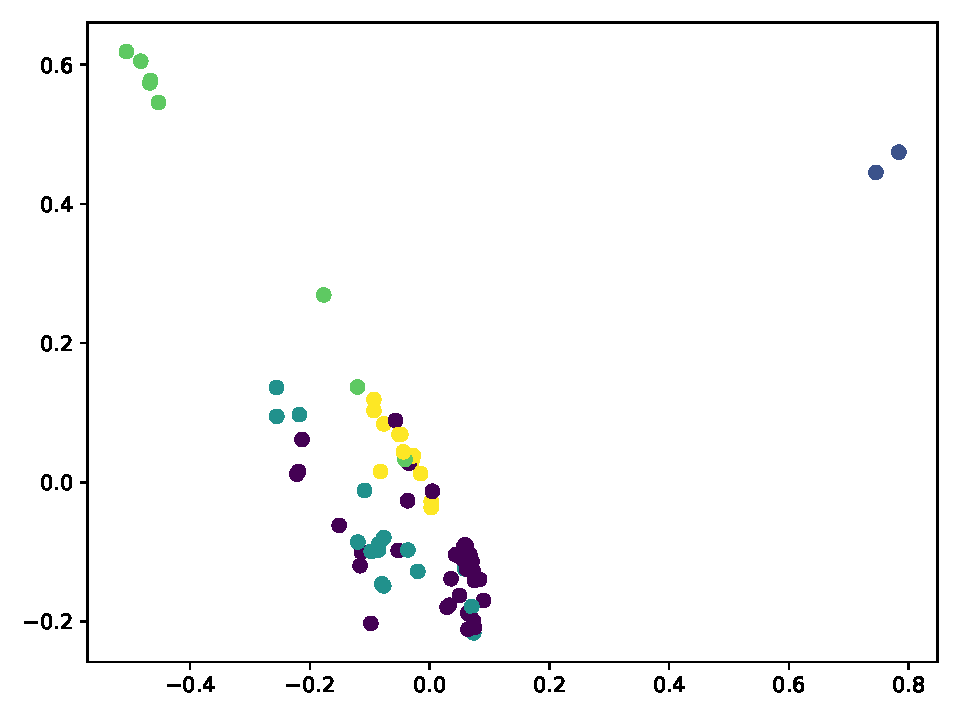
\includegraphics[width=\textwidth]{pca_1960-1975.pdf}
%   \caption{Data van 1960-1975.}
%   \label{fig:1960}
% \end{figure}

% \begin{figure}[H]
%   \centering
%   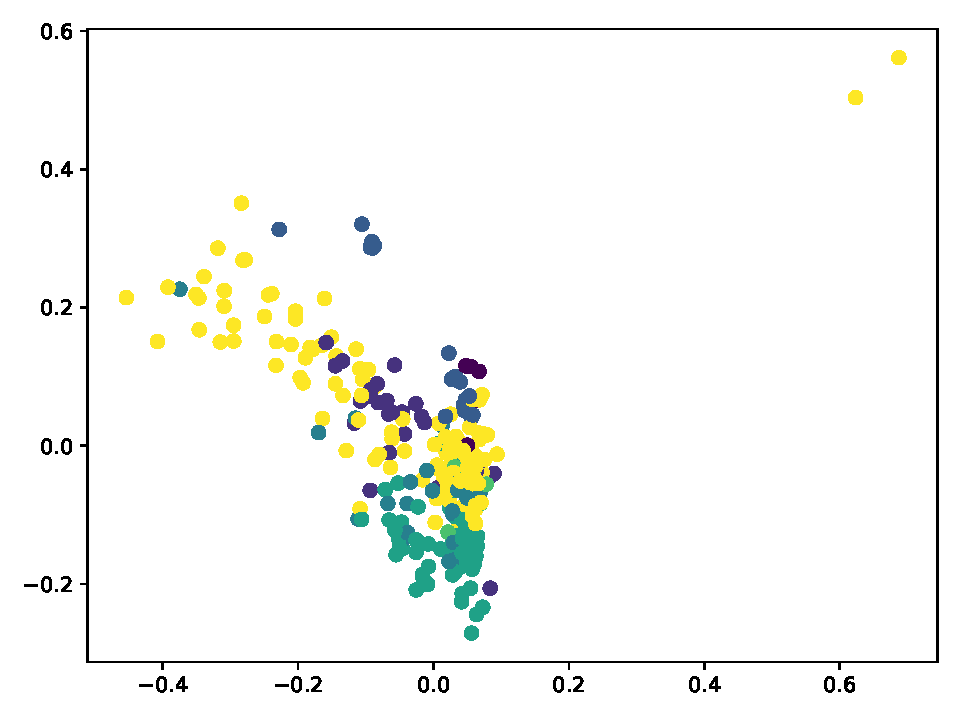
\includegraphics[width=\textwidth]{pca_1970-1985.pdf}
%   \caption{Data van 1970-1985.}
%   \label{fig:1970}
% \end{figure}

% \begin{figure}[H]
%   \centering
%   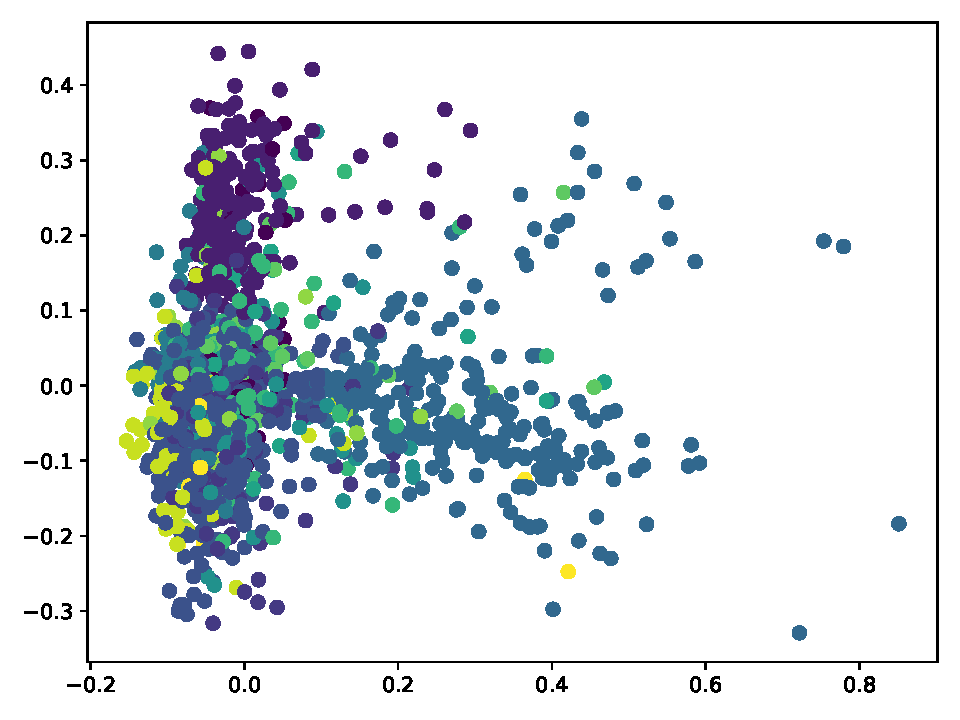
\includegraphics[width=\textwidth]{pca_1980-1995.pdf}
%   \caption{Data van 1980-1995.}
%   \label{fig:1980}
% \end{figure}

% \begin{figure}[H]
%   \centering
%   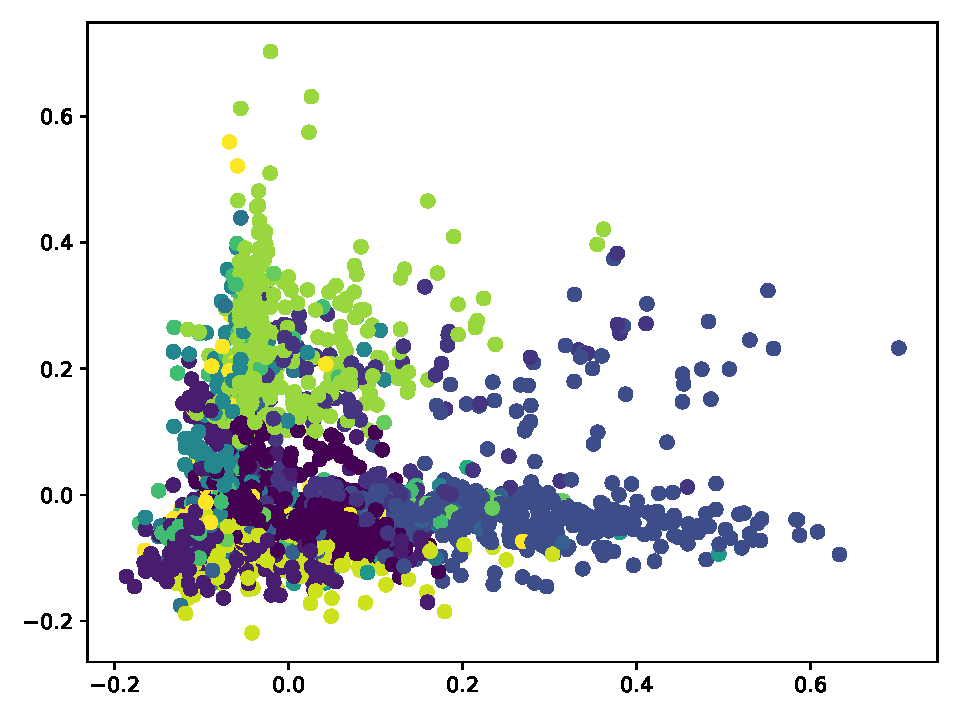
\includegraphics[width=\textwidth]{pca_1990-2005.pdf}
%   \caption{Data van 1990-2005.}
%   \label{fig:1990}
% \end{figure}

% \begin{figure}[H]
%   \centering
%   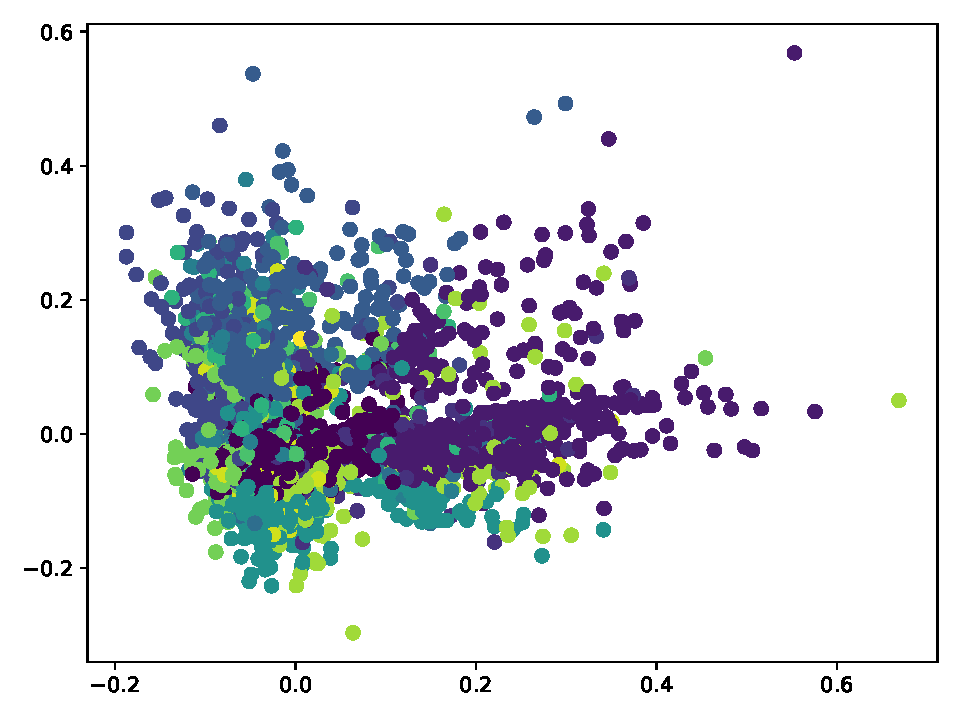
\includegraphics[width=\textwidth]{pca_2000-2015.pdf}
%   \caption{Data van 2000-2015.}
%   \label{fig:2000}
% \end{figure}

% \begin{figure}[H]
%   \centering
%   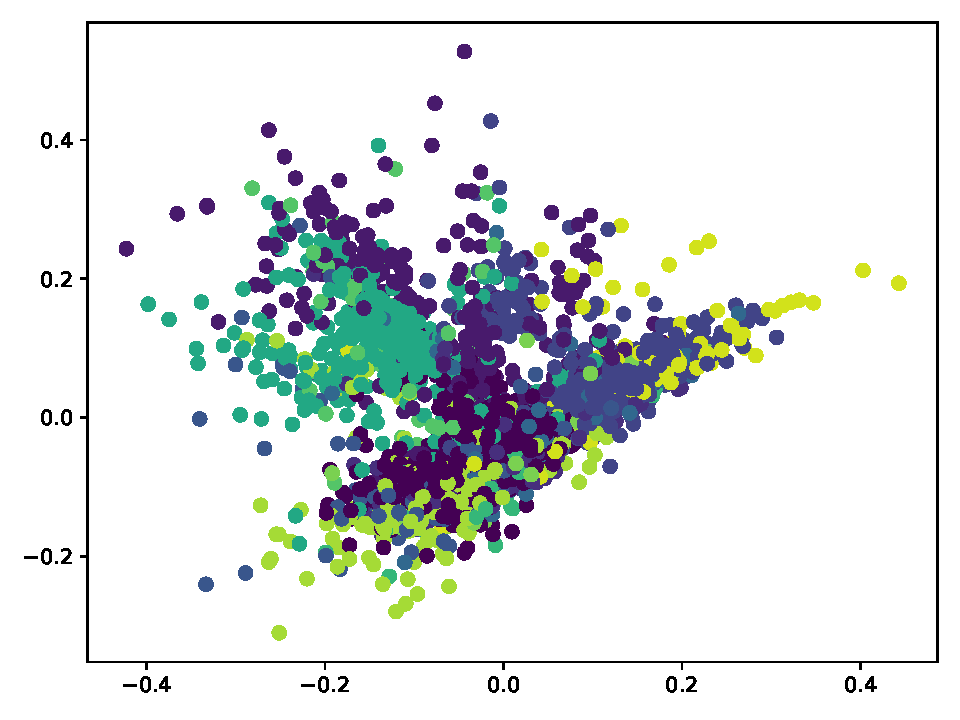
\includegraphics[width=\textwidth]{pca_2010-2025.pdf}
%   \caption{Data van 2010-2025.}
%   \label{fig:2010}
% \end{figure}


\appendix
  \section{Output van de KMeans clustering}
  \label{sec:output}
  \begin{lstlisting}[caption={KMeans output},label={lst:output},breaklines]

Clusters in range of year 1960 - 1975
88 titles in this range
Cluster 0: "Report to X3 on Data Definition Languages." - "ECMA: Preliminary Report on a Data Description Language." - "A Report on the CODASYL Meeting." - "Draft: Data Description Language." - "Program Portability, Data Manipulation Languages, and Data Description Languages." - 
Cluster 1: "Understanding Relations (Third Installment)." - "Understanding Relations (Installment #5)." - "Understanding Relations (Installment #4)." - "Understanding Relations." - "Understanding Relations." - 
Cluster 2: "Virtual Information in Data-Base Systems." - "Data Base Technical Conferences." - "Another Look at Data-Bases." - "Common Interface between Programming Languages abd Data Base Management Systems / Structured Programming and Integrated Data/Base Systems Design." - "Tutorial: What is a Data Base (from SIGBDP, SIGFIDET 1972)." - 
Cluster 3: "Call for Papers: 1972 ACM SIGFIDET Workshop on Data Description, Access and Control." - "1971 ACM-SIGFIDET Workshop on Data Description, Access and Control, Call for Papers" - "Call for Papers: ACM SIGFIDET Workshop on Data Description, Access and Control 1974." - "1971 ACM SIGFIDET Workshop on Data Description, Access and Control - Program." - "Final Program for 1972 ACM-SIGFIDET Workshop on Data Description, Access and Control." - 
Cluster 4: "First SIGFIDET Meeting, SJCC '69 / Second SIGFIDET Meeting, ACM '69." - "Report on SIGFIDET Meeting, SJCC, 1972." - "SIGFIDET Bibliography." - "A SIGFIDET Outline." - "SIGFIDET - A Statement of Scope." - 


Clusters in range of year 1970 - 1985
328 titles in this range
Cluster 0: "ACM SIGMOD Annual Business Meeting, 1974." - "ACM SIGMOD Annual Business Meeting 1976." - "ACM SIGMOD Annual Business Meeting, 1975." - "Letter to the Editor (implementation of RIGEL available)." - "The SIGFIDET Annual Business Meeting, August 28, 1973." - 
Cluster 1: "Comparison of Four Relational Data Model Specifications." - "Book Announcement: Data Models, by D. C. Tsichrittzis and F. H. Lochovsky." - "Towards a Data Model for Artificial Intelligence Applications." - "Molecular Objects, Abstract Data Types, and Data Models: A Framework." - "Comparison-Criteria for Semantic Data Models." - 
Cluster 2: "Call for Papers: 1972 ACM SIGFIDET Workshop on Data Description, Access and Control." - "Final Program for 1972 ACM-SIGFIDET Workshop on Data Description, Access and Control." - "1971 ACM-SIGFIDET Workshop on Data Description, Access and Control, Call for Papers" - "1971 ACM SIGFIDET Workshop on Data Description, Access and Control - Program." - "Call for Papers: ACM SIGFIDET Workshop on Data Description, Access and Control 1974." - 
Cluster 3: "Distributed Query Processing." - "Distributed Query Processing Strategies in Mermaid, A Frontend to Data Management Systems." - "Distributed Processing of Data Dynamics." - "DCT - A Testbed Approach to Distributed Systems Research." - "Distributed Query Optimization: An Engineering Approach." - 
Cluster 4: "On Some Metrics for Databases or What is a Very Large Database?" - "Time and Databases." - "A Note on Decompositions of Relational Databases." - "The Theory of Relational Databases." - "Errors in 'Process Synchronization in Database Systems'." - 
Cluster 5: "Entity-Relationship Model in the ANSI/SPARC Framework." - "An Algebra for a Directional Binary Entity-Relationship Model." - "An Entity-Relationship Algebra." - "A Modified Relational Algebra and its Use in an Entity-Relationship Environment." - "A Method for Optimization of a Conceptual Model." - 
Cluster 6: "Title, Table of Contents." - "Title, Table of Contents." - "Stable or Archival Tables." - 
Cluster 7: "Editor's Note." - "Research Directions in Data Base Management Systems." - "Research in Knowledge Base Management Systems." - "National Computer Conference 1975: Data Base Management." - "System/K: A Knowledge Base Management System." - 


Clusters in range of year 1980 - 1995
2553 titles in this range
Cluster 0: "Semantic Data Models." - "Semantic Data Engineering for Generalized Databases." - "Semantic Query Optimization in Recursive Databases." - "A Semantic Integrity Framework: Set Restrictions for Semantic Groupings." - "Logic-Based Approach to Semantic Query Optimization." - 
Cluster 1: "Distributed Query Processing." - "Query Processing for Temporal Databases." - "Query Processing Techniques in the Summary-Table-by-Example Database Query Language." - "Processing of Multiple Queries in Distributed Databases." - "Semantic Query Optimization for Tree and Chain Queries." - 
Cluster 2: "On the Data Model and Access Method of Summary Data Management." - "A Data Model and Access Method for Summary Data Management." - "Replicated Data Management in Distributed Database Systems." - "Data Management for Large Rule Systems." - "A Data/Knowledge Base Management Testbed and Experimental Results on Data/Knowledge Base Query and Update Processing." - 
Cluster 3: "Concurrency Control for Distributed Real-Time Databases." - "A Unified Concurrency Control Algorithm for Distributed Database Systems." - "A Paradigm for Concurrency Control in Heterogeneous Distributed Database Systems." - "Locking Protocols for Concurrency Control in Real-time Database Systems." - "An Adaptive Concurrency Control Strategy for Distributed Database Systems." - 
Cluster 4: " Object-Oriented Database System." - "Queries in Object-Oriented Databases." - "Object-Oriented Database Systems." - "A Model of Queries for Object-Oriented Databases." - "A Query Model for Object-Oriented Databases." - 
Cluster 5: "A Performance Evaluation of Four Parallel Join Algorithms in a Shared-Nothing Multiprocessor Environment." - "The Design and Implementation of a Parallel Join Algorithm for Nested Relations on Shared-Memory Multiprocessors." - "Architecture and Algorithm for Parallel Execution of a Join Operation." - "Multiprocessor Join Scheduling." - "Processor Scheduling for Multiprocessor Joins." - 
Cluster 6: "A Behaviour Integrated Entity-Relationship Approach for the Design of Object-Oriented Databases." - "The E-R Editor: an Editor for Database Conceptual Schema Design based on E-R Model." - "Supporting the Design of Conceptual Schemata by Database Systems." - "Entity-Relationship Consistency for Relational Schemas." - "A Conceptual Clustering Algorithm for Database Schema Design." - 
Cluster 7: "Constraint-Based Query Evaluation in Deductive Databases." - "On Semantic Query Optimization in Deductive Databases." - "A Rule-based Language for Deductive Object-Oriented Databases." - "Constraint-Based Reasoning in Deductive Databases." - "A Production Rule-Based Approach to Deductive Databases." - 
Cluster 8: "A Generalized Model for a Relational Temporal Database." - "A Relational Object Model." - "A Temporal Relational Algebra as Basis for Temporal Relational Completeness." - "A Homogeneous Relational Model and Query Languages for Temporal Databases." - "Incomplete Information in Relational Temporal Databases." - 
Cluster 9: "Database Programming in Transaction Logic." - "Database Programming Languages: A Functional Approach." - "The O++ Database Programming Language: Implementation and Experience." - "Towards a Logical-Object Oriented Programming Language for Databases." - "Types and Persistence in Database Programming Languages." - 
Cluster 10: "Dynamic Voting." - "Distributed Processing of Data Dynamics." - "Efficient Dynamic Voting Algorithms." - "Dynamics Analysis in Database Design." - "Dynamic Hashing Schemes." - 
Cluster 11: "A Performance Evaluation of Multi-Level Transaction Management." - "Performance Evaluation of a Temporal Database Management System." - "Performance Modeling of Distributed Database." - "Database Mining: A Performance Perspective." - "Scheduling Real-time Transactions: a Performance Evaluation." - 
Cluster 12: "Research Directions for Distributed Databases." - "Research Directions in Object-Oriented Database Systems." - "Database Research at the IBM Almaden Research Center." - "Object-Oriented Databases: Definition and Research Directions." - "Research Issues in Spatial Databases." - 


Clusters in range of year 1990 - 2005
5002 titles in this range
Cluster 0: "Database Mining: A Performance Perspective." - "A Rule-Based Approach for the Design and Implementation of Information Systems." - "Tree-Based Access Methods for Spatial Databases: Implementation and Performance Evaluation." - "Active Database Systems: Triggers and Rules For Advanced Database Processing." - "Distributed Rule Processing in Active Databases." - 
Cluster 1: "Minimizing Detail Data in Data Warehouses." - "A Data Model and Data Structures for Moving Objects Databases." - "Data Organization and Access for Efficient Data Mining." - "Multidimensional Data Modeling for Complex Data." - "Simulation data as data streams." - 
Cluster 2: "A Temporal Model and Query Language for ER Databases." - "TOOSQL - A Temporal Object-Oriented Query Language." - "From a Database Programming Language to a Database Specification Language (Invited Paper)." - "Object Queries over Relational Databases: Language, Implementation, and Applications." - "A Temporal Query Language Based on Conceptual Entities and Roles." - 
Cluster 3: "A Query Model for Object-Oriented Databases." - "Object Placement in Parallel Object-Oriented Database Systems." - "A Model for Active Object Oriented Databases." - "Semantic Query Processing in Object-Oriented Database Systems." - "Querying Object-Oriented Databases." - 
Cluster 4: "Matching Large XML Schemas." - "Database Schema Evolution through the Specification and Maintenance of Changes on Entities and Relationships." - "Mapping an Extended Entity-Relationship Schema into a Schema of Complex Objects." - "A Transparent Object-Oriented Schema Change Approach Using View Evolution." - "Integration of Heterogeneous Object Schemas." - 
Cluster 5: "Composing Web services on the Semantic Web." - "A Conceptual Architecture for Semantic Web Enabled Web Services." - "Pi-Web Join in a Web Warehouse." - "The Web as a Graph." - "Web Information Retrieval." - 
Cluster 6: "Fast Joins Using Join Indices." - "Spatial Join Indices." - "Review - Fast Joins Using Join Indices." - "Spatial Joins and R-trees." - "Evaluation of Main Memory Join Algorithms for Joins with Set Comparison Join Predicates." - 
Cluster 7: "Research Directions for Distributed Databases." - "Research Directions in Object-Oriented Database Systems." - "Research Issues in Spatial Databases." - "Database Research at the University of Florida." - "Database Research at the IBM Almaden Research Center." - 
Cluster 8: "What Will Be - Book Review." - "Call for Book Reviews." - "Book Review Column." - "Book review column." - "Book Review Column." - 
Cluster 9: "Efficient Storage of XML Data." - "Efficient Indexing for Constraint and Temporal Databases." - "Efficient OLAP Query Processing in Distributed Data Warehouses." - "Efficient OLAP Query Processing in Distributed Data Warehouse." - "Efficient Processing of Proximity Queries for Large Databases." - 
Cluster 10: "Query Optimization in a Heterogeneous DBMS." - "Alert: An Architecture for Transforming a Passive DBMS into an Active DBMS." - "Land below a DBMS." - "Implementation Aspects of an Object-Oriented DBMS." - "Implementing High Level Active Rules on Top of a Relational DBMS." - 
Cluster 11: "Processing Top N and Bottom N Queries." - "Dynamic Query Optimization and Query Processing in Multidatabase Systems." - "XML Query Processing and Optimization." - "A Graph Query Language and Its Query Processing." - "Distributed Query Optimization by Query Trading." - 
Cluster 12: "Scientific Workflow Management by Database Management." - "Multimedia Database Management Systems." - "The MARIFlow Workflow Management System." - "Extensible Database Management Systems." - "Data Management for Large Rule Systems." - 
Cluster 13: "What's Next in XML and Databases?" - "Management of XML Documents in Object-Relational Databases." - "XML-Based Applications Using XML Schema." - "XML schema." - "Querying XML Data." - 


Clusters in range of year 2000 - 2015
5858 titles in this range
Cluster 0: "Index-Based Keyword Search in Mediator Systems." - "Scalable ontology-based information systems." - "Network-Based Problem Detection for Distributed Systems." - "Model-based approximate querying in sensor networks." - "Keyword-based correlated network computation over large social media." - 
Cluster 1: "Data Stream Query Processing." - "XML Query Processing and Optimization." - "Dynamic Query Optimization and Query Processing in Multidatabase Systems." - "A Query Processing Mechanism for Top-k Query in P2P Networks." - "Top-k Query Processing in Uncertain Databases." - 
Cluster 2: "Join Reordering by Join Simulation." - "Hash-Merge Join: A Non-blocking Join Algorithm for Producing Fast and Early Join Results." - "Top-k Set Similarity Joins." - "The similarity join database operator." - "Efficient Temporal Join Processing Using Indices." - 
Cluster 3: "Optimizing Timestamp Management in Data Stream Management Systems." - "Data Management in the Cloud." - "Data Management in the Social Web." - "Issues in data stream management." - "Flexible Dataspace Management Through Model Management." - 
Cluster 4: "Simulation data as data streams." - "RFID Data Processing with a Data Stream Query Language." - "Building data warehouses with semantic data." - "Data Stream Sharing." - "Scaling Clustering Algorithms for Massive Data Sets using Data Streams." - 
Cluster 5: "XML schema." - "Matching Large XML Schemas." - "How schema independent are schema free query interfaces?" - "A Tale of Two Schemas: Creating a Temporal XML Schema from a Snapshot Schema with tXSchema." - "Schema and Data Translation." - 
Cluster 6: "A data mining proxy approach for efficient frequent itemset mining." - "Mining Views: Database Views for Data Mining." - "Mining Web Structures Using Multi-Dimensional Data Mining Model." - "Mining Software Data." - "-anonymity in data mining." - 
Cluster 7: "Using XML to Build Efficient Transaction-Time Temporal Database Systems on Relational Databases." - "A Database Approach to Quality of Service Specification in Video Databases." - "Efficient query evaluation on probabilistic databases." - "Querying Graph Databases." - "Query languages for graph databases." - 
Cluster 8: "Optimizing ETL Processes in Data Warehouses." - 
Cluster 9: "Privacy-Preserving Top-K Queries." - "Privacy-Preserving Data Mining." - "Privacy Preserving Joins." - "Privacy-preserving data publishing." - "Privacy-preserving data mashup." - 
Cluster 10: "On High Dimensional Skylines." - "Discovery of High-Dimensional." - "On High Dimensional Indexing of Uncertain Data." - "Querying high-dimensional data in single-dimensional space." - "High-dimensional similarity retrieval using dimensional choice." - 
Cluster 11: "Composing Web services on the Semantic Web." - "A Conceptual Architecture for Semantic Web Enabled Web Services." - "The Web as a Graph." - "Top-k queries over web applications." - "The hidden web, XML and the Semantic Web: scientific data management perspectives." - 
Cluster 12: "What's Next in XML and Databases?" - "XML-Based Applications Using XML Schema." - "XML Query Processing." - "Updates on XML documents and schemas." - "Classification and Querying of XML Documents." - 
Cluster 13: "An Efficient Graph Indexing Method." - "Graph indexing for reachability queries." - "Efficient Indexing of Spatiotemporal Objects." - "Indexing relations on the web." - "Indexing Incomplete Databases." - 
Cluster 14: "Indexing Multidimensional Time-Series." - "Querying time-series streams." - 


Clusters in range of year 2010 - 2025
5512 titles in this range
Cluster 0: "Efficient structural graph clustering: an index-based approach." - "GLog: A high level graph analysis system using MapReduce." - "Towards Efficient Motif-based Graph Partitioning: An Adaptive Sampling Approach." - "A model-based approach for text clustering with outlier detection." - "Efficient Team Formation in Social Networks based on Constrained Pattern Graph." - 
Cluster 1: "Efficient Continuous Multi-Query Processing over Graph Streams." - "Towards Flexible Event Processing in Distributed Data Streams." - "Robust distributed stream processing." - "Efficient Stream Processing of Scientific Data." - "Benchmarking Distributed Stream Data Processing Systems." - 
Cluster 2: "Automated Machine Learning for Entity Matching Tasks." - "Data Curation with Deep Learning." - "Automatic View Generation with Deep Learning and Reinforcement Learning." - "Adaptive Dynamic Bipartite Graph Matching: A Reinforcement Learning Approach." - "Workload management for cloud databases via machine learning." - 
Cluster 3: "Distance-Based Data Mining over Encrypted Data." - "Automated Data Science for Relational Data." - "A system for energy-efficient data management." - "Scalable data management: NoSQL data stores in research and practice." - "Building data warehouses with semantic data." - 
Cluster 4: "Top-k graph pattern matching over large graphs." - "Efficient and Effective Community Search on Large-scale Bipartite Graphs." - "Large-scale spatial join query processing in Cloud." - "Graph databases for large-scale healthcare systems: A framework for efficient data management and data services." - "Multi-Constrained Graph Pattern Matching in large-scale contextual social graphs." - 
Cluster 5: "Privacy-preserving data publishing." - "Privacy-Integrated Graph Clustering Through Differential Privacy." - "A privacy framework: indistinguishable privacy." - "Privacy Preserving Similarity Evaluation of Time Series Data." - "Algorithm-safe privacy-preserving data publishing." - 
Cluster 6: "Multiscale Frequent Co-movement Pattern Mining." - 
Cluster 7: "Evaluating List Intersection on SSDs for Parallel I/O Skipping." - 
Cluster 8: "Correction: A survey of community search over big graphs." - "A survey of community search over big graphs." - 
Cluster 9: "Query languages for graph databases." - "Why-query support in graph databases." - "Query Games in Databases." - "Learning Path Queries on Graph Databases." - "Efficient query answering against dynamic RDF databases." - 
Cluster 10: "Towards Visualization Recommendation Systems." - "Event Recommendation using Social Media." - "Ontology-based news recommendation." - "Online Social Media Recommendation Over Streams." - "A general graph-based model for recommendation in event-based social networks." - 
Cluster 11: "Skyline queries, front and back." - "Top-k Skyline Groups Queries." - "SkyEngine: Efficient Skyline search engine for Continuous Skyline computations." - "Efficient Skyline Computation in MapReduce." - "Efficient Computation of G-Skyline Groups (Extended Abstract)." - 
Cluster 12: "Towards Scalable Data Discovery." - "Efficient Discovery of Approximate Order Dependencies." - "Approximate Order Dependency Discovery." - "Aurum: A Data Discovery System." - "Distributed Discovery of Functional Dependencies." - 
Cluster 13: "Keyword Search on Temporal Graphs." - "Scalable top-k spatial keyword search." - "Keyword-based search and exploration on databases." - "Top-k keyword search over probabilistic XML data." - "Scalable keyword search on large data streams." - 
Cluster 14: "Big data integration." - "Real-Time Data Management for Big Data." - "Workload management for Big Data analytics." - "Machine learning on Big Data." - "How Different is Big Data?" - 
Cluster 15: "Histogramming Privately Ever After: Differentially-Private Data-Dependent Error Bound Optimisation." - 
\end{lstlisting}

\end{document}

%%% Local Variables:
%%% mode: latex 
%%% TeX-master: t
%%% End: